\chapter{Introduction}
Microfluidics is the science of handling and manipulating very small volumes of fluids. It is a multidisciplinary field that involves engineering, physics, chemistry, biochemistry, nanotechnology, and biotechnology. Microfluidic biochips combine different biochemical analysis functionalities, e.g. mixers, filter, detectors, on-chip. It miniaturises the macroscopic chemical and biological processes to a sub-millimetre scale \cite{microfluidic-largescale}.  
\\
There are several types of microfluidic biochip platforms. Based on the fluid manipulation on the chip, biochips can broadly be divided into two categories \cite{wajid}.
\begin{itemize}
\item Droplet-based biochips
\item Flow-based biochips
\end{itemize}
In this thesis the focus is on flow-based biochips. The following sections will explain the flow-based technology and its application areas.

\section{Flow-based Biochips}
Flow-based biochips are fabricated using multilayer soft lithography. \autoref{fig:flow-based-biochip} shows a flow-based biochip. Polydimethylsiloxane, \emph{PDMS}, is used as the fabrication substrate \cite{integration-microfluidics}. PDMS is used as it is a cheap and rubber-like elastomer with good biocompatibility and optical transparency.
\begin{figure}[H]
\centering
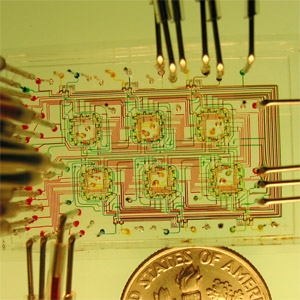
\includegraphics[scale=0.65]{figures/flow-based-biochip.jpg}
\caption[Flow-based biochip]{Flow-based biochip \cite{stanford-group}.}
\label{fig:flow-based-biochip}
\end{figure}

Flow-based biochips can have multiple physical layers, but the layers are logically divided into two types: \emph{flow layer} and \emph{control layer}. The flow layer is depicted in blue and the control layer in red as shown in \autoref{fig:flow-based-concept}a. The liquid is in the flow layer and it is manipulated using the control layer \cite{integration-microfluidics}.

\begin{figure}[H]
\centering
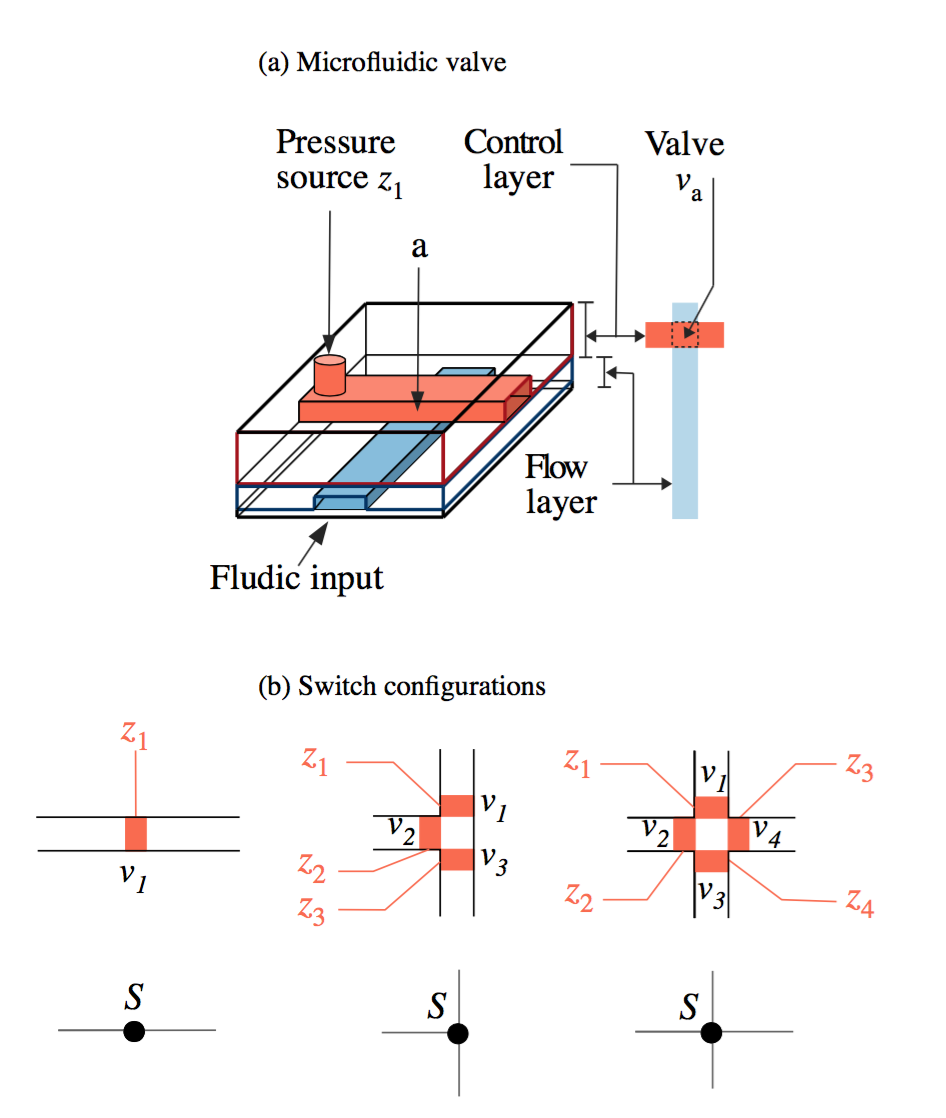
\includegraphics[scale=0.425]{figures/flow-based-concept.png}
\caption[Flow-based valve and switch]{Flow-based valve and switch \cite{wajid}.}
\label{fig:flow-based-concept}
\end{figure}

A valve (shown in \autoref{fig:flow-based-concept}a) is the basic building block of such a biochip. The control layer is connected to an external air pressure source through the punch hole $z_1$. This is referred to as a control pin. The flow layer is connected to a fluid reservoir through a pump which generates the fluid flow. When the external air pressure in the control layer is not active, the fluid is permitted to flow freely, i.e. the valve is open. When the pressure source is activated, the high pressure causes the elastic control layer to pinch the underlying flow layer (point $a$ in \autoref{fig:flow-based-concept}a) blocking the fluid flow, i.e. the valve is closed. These valves are used to manipulate fluids in the flow layer as the valves either restrict or permit the fluid flow. More complex units such as switches, mixer, micropumps, etc., can be formed by combining these valves. An example of valves combining to form a component is that of a switch. Three different switch configurations are depicted in \autoref{fig:flow-based-concept}b. As shown here a switch can consist of one or more valves. Multiple valve switches are present at channel junctions and are used to control the path of the fluids entering the switch from different sides. The fluid flow can be generated by either using off-chip or on-chip pumps. The control layer is not necessarily above the flow layer as shown in \autoref{fig:flow-based-concept}a. It can also be below the flow layer by creating a "push-up" valve, and having the control layer above the flow layer is done by creating a "push-down" valve. The connections to external ports (fluidic ports for the flow layer and pressure sources for the control layer) are made by punching holes in the chip and placing external tubings into the punch holes \cite{integration-microfluidics}. All input ports are connected to the off-chip pumps.

\subsection{Application Areas}
Since the introduction of this technology, several biochips have been designed which target a variety of biochemical applications \cite{life-sciences-microfluidics}. A few are listed below:

\begin{itemize}
\item \emph{Microreaction Technology}: These chips allow the production of fine chemicals. The superior mixing and reaction control properties of microfluidic systems are used to perform chemical reaction or syntheses at much better yields and better selectivity than in conventional systems. Chemical reactions can take place much faster by reducing the diffusion length \cite{life-sciences-microfluidics}.

\item \emph{Cell Biology}: As the typical dimensions of cells are 5-20 $\mu m$, it is an ideal size for the size range of typical microfluidic structures. The applications within cell biology range from the observation of the physical and biological behaviour of single cells in different culturing media, chemotaxis experiments to observations of growth patterns, the guidance of growth. This can potentially be of great importance in drug research \cite{life-sciences-microfluidics}.

\item \emph{Diagnosis Testing}: Certain chips allow the diagnosis of diseases. Known examples are chips testing for Human Immunodeficiency Virus (\emph{HIV}) and syphilis \cite{wajid}. The chip designed for this purpose is cheap, easy to use, requires only micro-litres of the blood sample and it simultaneously tests for HIV and syphilis producing the result within 20 minutes \cite{wajid}.

\end{itemize}


One of the biggest beneficiaries of microfluidic devices and systems is the diagnostic market, especially molecular diagnostics. Microfluidics and miniaturisation technologies have a crucial enabling role for new product development in this field due to the required integration density, portability and speed for such applications can only be realised in miniaturised solutions. Additionally, many of the diagnostic procedures require the integration of methods of molecular biology like DeoxyriboNucleic Acid (DNA) extraction or Polymerase Chain Reaction (PCR) which can only be performed in their microfluidics-based protocols outside a specialised laboratory \cite{life-sciences-microfluidics}.

\section{Motivation}
A potential roadblock in the deployment of microfluidic biochips is the lack of test techniques to screen defective devices before they are used for biochemical analysis. Defective chips lead to repetition of experiments. This is undesirable due to high reagent cost and limited availability of samples. %Flow-based biochips are also affected by faults, and the defects can escape the after-fabrication inspection and can thereby affect the operation.
Recent work has addressed the fault-modeling and the automated testing of flow-based biochips \cite{fault-modeling}.

Based on these fault models and testing techniques, the objective of this thesis is to propose approaches for the fault-tolerant design of flow-based biochips, such that the biochips can tolerate several permanent faults, given a cost budget and a biochip area. During the physical design of the biochip layout, redundancy can be introduced for on-chip components such as valves, channels and microfluidic units to improve fault-tolerance, thereby increasing thus the yield.

This thesis explores techniques and algorithms for designing fault-tolerant flow-based biochips. The purpose is to design and implement a tool to assist the designer in designing a fault-tolerant biochip. Implementing such a tool requires a biochip architecture model, biochemical application model, heuristics for introducing fault-tolerance and a way to evaluate the fault-tolerance of the biochip.
%The remaining chapters elaborate these topics, formulate the exact problem, and evaluate the tool on a set of benchmarks.

\subsection{Related Work}
In \cite{wajid} there are proposed system models for flow-based biochips which are used in this thesis. The proposed models used in this thesis are the biochip architecture model and the biochemical application model. Additionally, \cite{wajid} also contributes towards application mapping, architectural synthesis and control synthesis for flow-based biochips.

The physical placement of components is done by the designer of the flow-based biochip, which is a time-consuming and error-prone phase. In \cite{michael}, an automated tool for the physical placement of components is proposed which assists the designer in choosing the best placement.

Fault-tolerant design of microfluidic biochips has been done in \cite{mirela}. However, the thesis in \cite{mirela} introduces fault-tolerant design for droplet-based biochips. The thesis proposes algorithms to generate application-specific biochip architectures that are able to tolerate a certain number of permanent faults. The aim of the thesis was to increase the yield of fabricated biochips.


\section{Thesis Overview}
This thesis is organised in eight chapters. A brief summary of the chapters are provided here.

\begin{description}
\item[Chapter 2] presents the different types of faults in flow-based biochips and an automated testing strategy to determine the faults and locations thereof in a flow-based biochip.

\item[Chapter 3] describes the system models used in this thesis and proposes a fault-model for flow-based biochips. Furthermore it outlines the problem of application mapping.

\item[Chapter 4] focuses on the fault-tolerant architecture synthesis problem for flow-based biochips. It proposes two algorithmic solutions to obtain a fault-tolerant architecture.

\item[Chapter 5] proposes an evaluation method for architectures in order to determine if a given architecture is fault-tolerant.

\item[Chapter 6] describes the implementation of the tool developed in this thesis.

\item[Chapter 7] experimentally evaluates the proposed algorithmic approaches on a number of benchmarks. The evaluation is done in terms of solution quality and performance of the algorithms.

\item[Chapter 8] presents the conclusions of this thesis and the options for future work.

\end{description}